\documentclass{article}
\usepackage[margin=2cm]{geometry}
\usepackage{graphicx}
\usepackage{tikz}
\usetikzlibrary {trees,graphs,3d,positioning}
\usepackage{xkcdcolors}
\usepackage{pgfplots}
\pgfplotsset{compat=1.5}
\usepackage{physics}
\usepackage{xparse}
\usepackage{siunitx}

\begin{document}
\section{Materials}
Snap Fastener

\section{Classical Cryptography exercises}
\subsection{Caesar cipher - A type of substitution cipher}
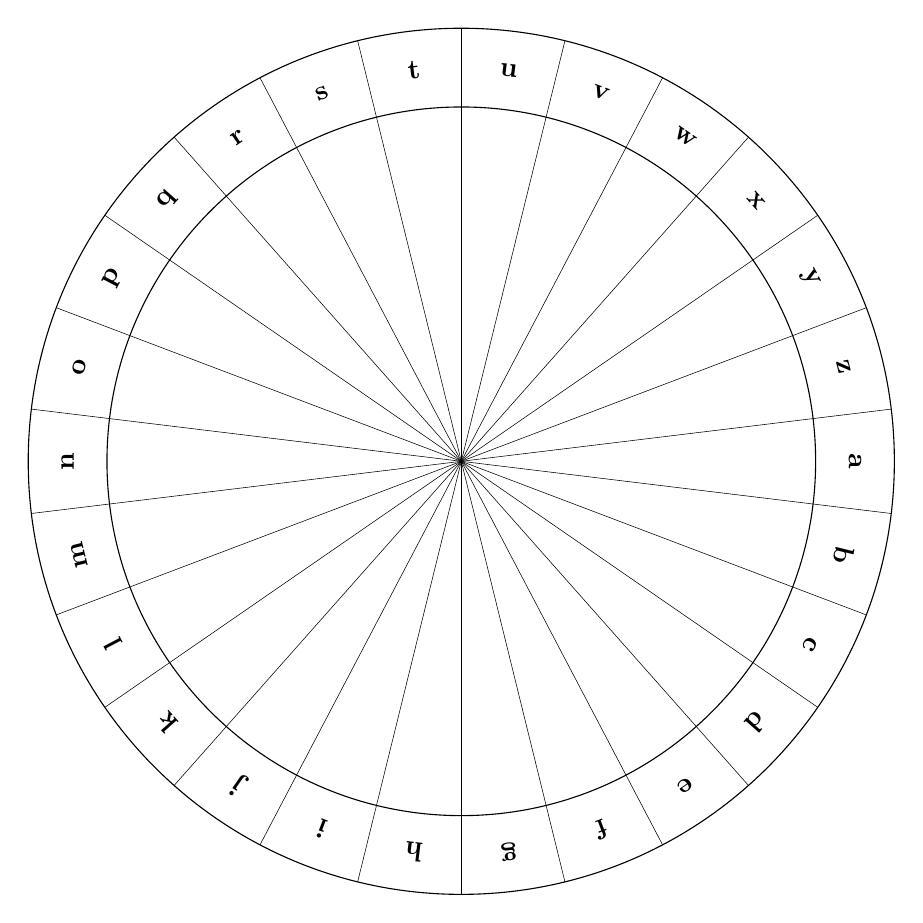
\begin{tikzpicture}
\pgfmathsetmacro{\a}{360/26}
\foreach \letter [count=\i from 0] in {a,...,z} {
    \node[rotate={-\i*\a-90}] at ({-\i*\a}:5) {\textbf\letter};
    \draw[very thin] (0,0) -- ({(\i+.5)*\a}:5.5); 
}
\draw (0,0) circle [radius=5.5];
\draw (0,0) circle [radius=4.5];
\end{tikzpicture}

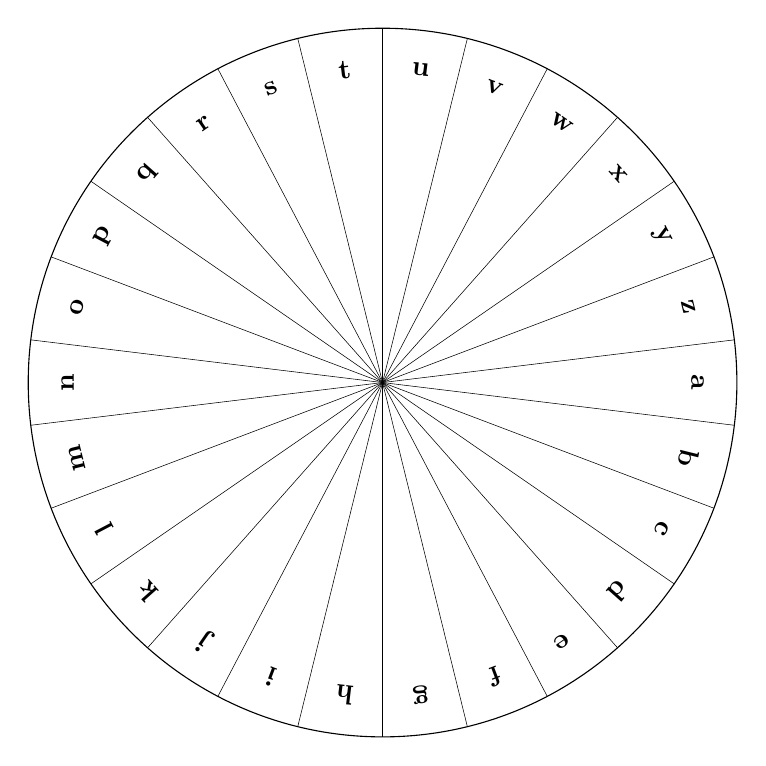
\begin{tikzpicture}
\pgfmathsetmacro{\a}{360/26}
\foreach \letter [count=\i from 0] in {a,...,z} {
    \node[rotate={-\i*\a-90}] at ({-\i*\a}:4) {\textbf\letter};
    \draw[very thin] (0,0) -- ({(\i+.5)*\a}:4.5); 
}
\draw (0,0) circle [radius=4.5];
\end{tikzpicture}

Build your own

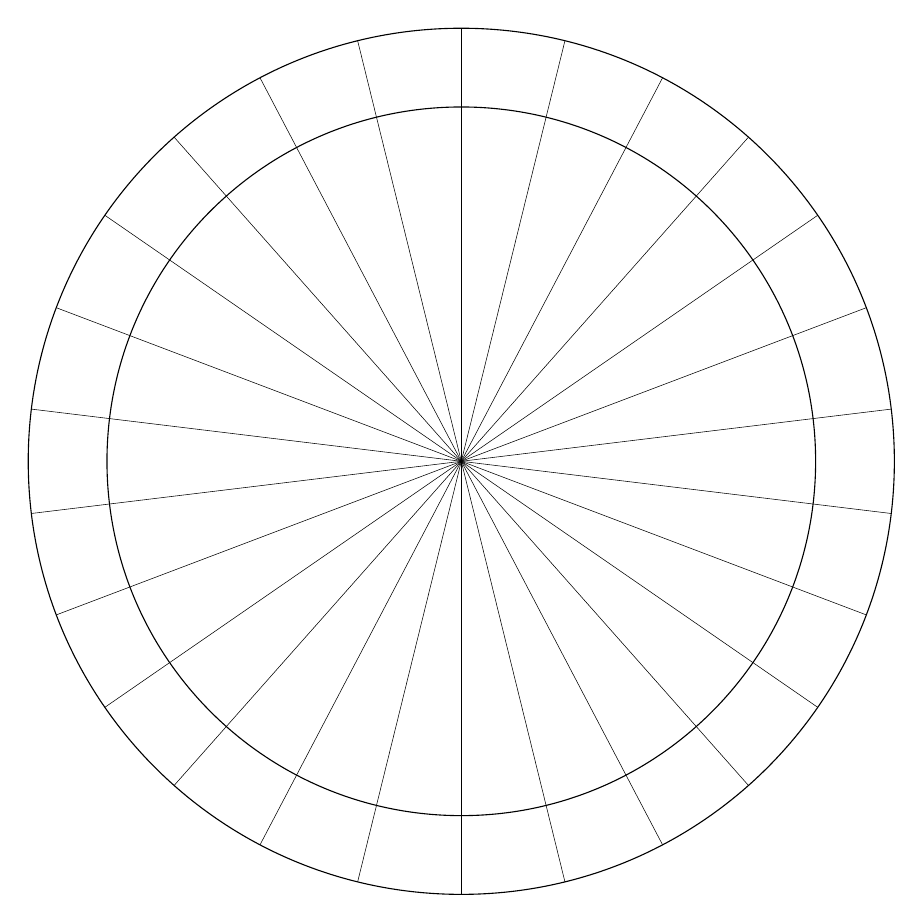
\begin{tikzpicture}
\pgfmathsetmacro{\a}{360/26}
\foreach \letter [count=\i from 0] in {a,...,z} {
    % \node[rotate={-\i*\a-90}] at ({-\i*\a}:5) {\textbf\letter};
    \draw[very thin] (0,0) -- ({(\i+.5)*\a}:5.5); 
}
\draw (0,0) circle [radius=5.5];
\draw (0,0) circle [radius=4.5];
\end{tikzpicture}

\begin{enumerate}
    \item Hohphqwdub, pb ghdu Zdwvrq
    \item Bw mdmzg ikbqwv bpmzm qa iteiga iv mycit ivl wxxwaqbm zmikbqwv
    \item Evmvi crlxy rk czmv uirxfej
    \item Hdojxcjiymdv dn ocz kjrzmcjpnz ja ocz xzgg
\end{enumerate}
\begin{enumerate}
    \item (3) Elementary, my dear Watson
    \item (8) To every action there is always an equal and opposite reaction
    \item (17) Never laugh at live dragons.
    \item (21) Mitochondria is the powerhouse of the cell
\end{enumerate}
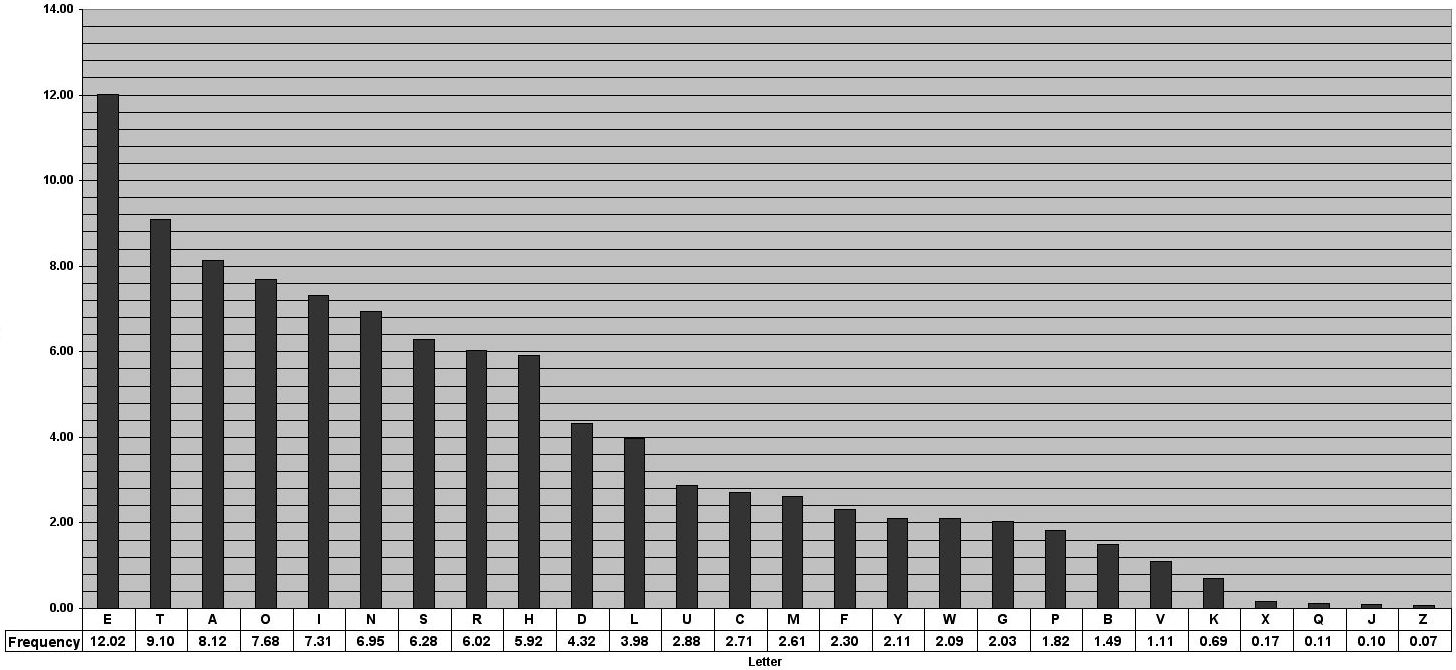
\includegraphics[width=\textwidth]{letter_frequency}
English Letter Frequency (based on a sample of 40,000 words)
https://pi.math.cornell.edu/~mec/2003-2004/cryptography/subs/frequencies.html
\subsection{QR code}
\section{Concept}
Light is made of photons. It is an em wave with a polarization. 
\subsection{Light as a wave}
Has a defined frequency and wavelength, delocalized, interference phenomenon
\subsection{Light as a particle}
Photoelectric effect, made of chunks called photons.

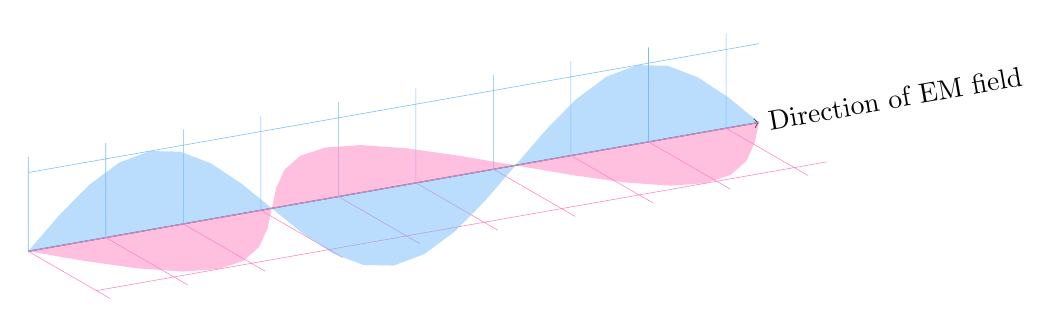
\begin{tikzpicture}[x={(10:10mm)},z={(-30:10mm)},domain=0:3*pi]
    \draw[->] (0,0) -- (3*pi,0) node[right,rotate=10] {Direction of EM field};
    % \draw[->] (0,0) -- (0,1.2) node[right] {$y$};
    % \draw[->] (0,0) -- (0,0,1.2) node[right] {$x$};
    \begin{scope}[canvas is xy plane at z=0]
    \draw[very thin,xkcdSkyBlue] (0,0) grid (3*pi,1.2);
    \end{scope}
    \begin{scope}[canvas is xz plane at y=0]
    \draw[very thin,xkcdPink] (0,0) grid (3*pi,1.2);
    \end{scope}
    \fill[color=xkcdSkyBlue,fill opacity=0.5] plot (\x,{sin(\x r)});
    \fill[color=xkcdPink,fill opacity=0.5] plot (\x,0,{sin(\x r)});
\end{tikzpicture}

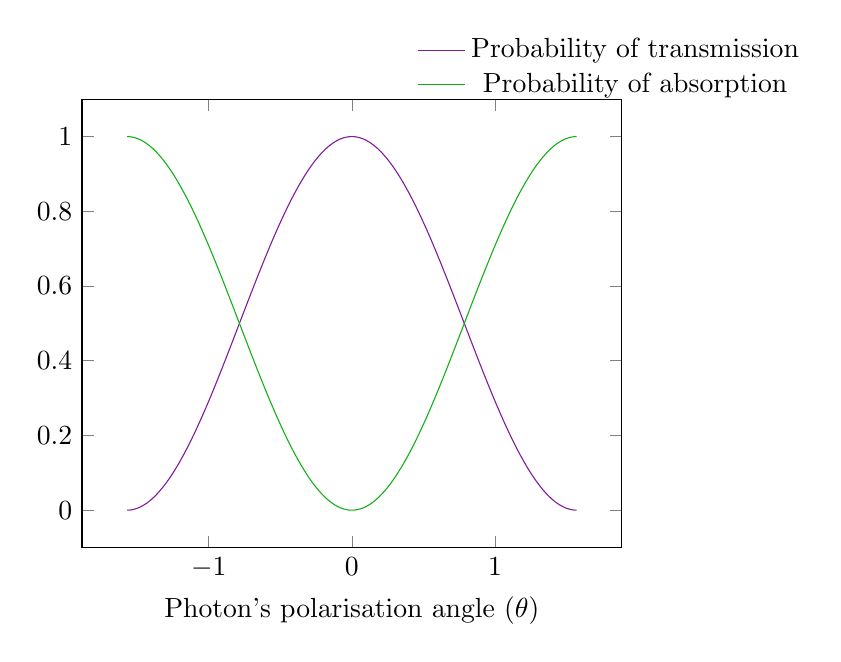
\begin{tikzpicture}
\begin{axis}[
    xlabel={Photon's polarisation angle ($\theta$)},
        legend style={
        anchor=south,
        draw=none,
        fill=none,
    },
]
\addplot[xkcdPurple, domain={-pi/2:pi/2}, samples=200]
    {cos(deg(x))^2};
\addlegendentry{Probability of transmission}
\addplot[xkcdGreen, domain={-pi/2:pi/2}, samples=200]
    {sin(deg(x))^2};
\addlegendentry{Probability of absorption}
\end{axis}
\end{tikzpicture}


The direction of the electric field is called the light's polarization.

Polarizers are special sheets of material that absorb or transmit
light depending on its polarization.

Consider a single photon at a polarizer. There are only two possible things that can happen:
A. The photon goes through;
B. The photon is absorbed

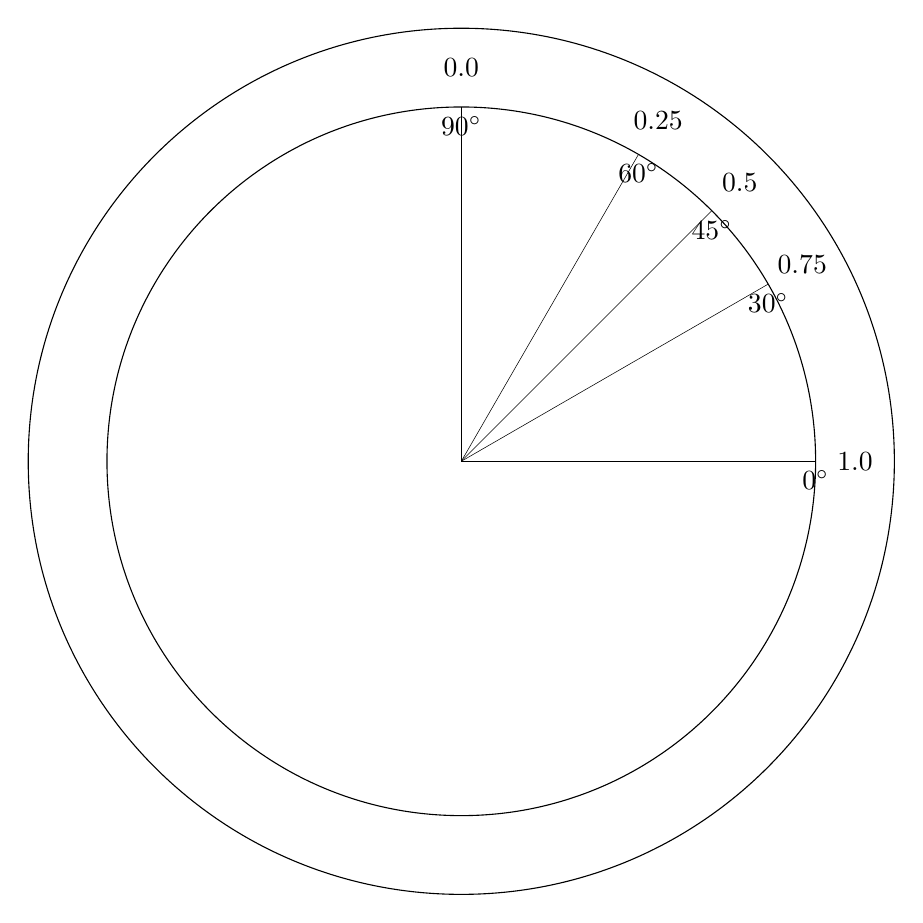
\begin{tikzpicture}
\foreach \a [count=\i from 0] in {0, 30, 45, 60, 90} {
\pgfmathsetmacro{\t}{cos(\a)^2};
\node[rotate={0}] at ({\a}:5) {\t};
    \draw[very thin] (0,0) -- (\a:4.5) node[below] {\ang{\a}}; 
}
\draw (0,0) circle [radius=5.5];
\draw (0,0) circle [radius=4.5];
\end{tikzpicture}

Mutually exclusive

Vertical and Horizontal are mutually exclusive

vertical and diagonal (\ang{45}) polarizations are not mutually exclusive

\ang{45} and -\ang{45} polarizations are mutually exclusive

Any two perpendicular polarizations are mutually exclusive.

\subsection{Superposition}
A quantum object can be in a superposition of multiple states at once. For example, a +\ang{45}-polarized photon is in a superposition of horizontal and vertical polarization states.

\subsection{Measurement}

Superposition works as long as you don't look! The act of measuring the superposition will collapse it and change the state. For example, when we measure the +\ang{45}-polarized photon in the HV basis, it must collapse to either horizontal or vertical polarization

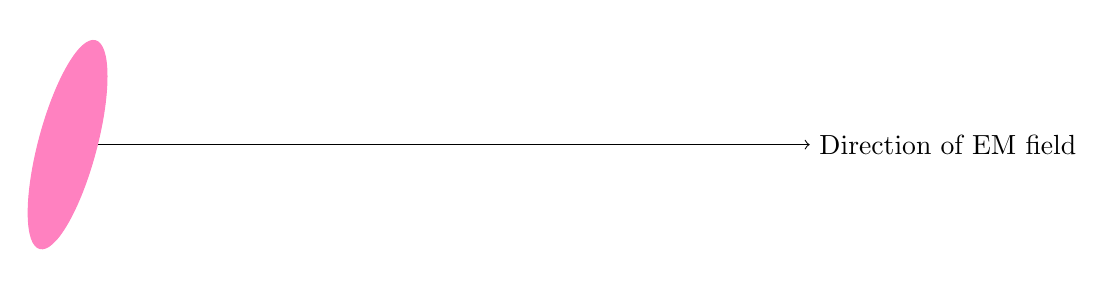
\begin{tikzpicture}[x={(90:10mm)},y={(-120:10mm)},z={(0:10mm)},domain=0:3*pi]
    \draw[->] (0,0,0) -- (0,0,3*pi) node[right,rotate=0] {Direction of EM field};
    % \draw[->] (0,0) -- (0,1.2) node[right] {$y$};
    % \draw[->] (0,0) -- (0,0,1.2) node[right] {$x$};
    \begin{scope}[canvas is xy plane at z=0]
    % \draw[very thin,xkcdSkyBlue] (0,0) grid (3*pi,1.2);
    \filldraw[color=xkcdPink] (0,0) circle [radius=1cm];
    \end{scope}
    % \begin{scope}[canvas is xz plane at y=0]
    % \draw[very thin,xkcdPink] (0,0) grid (3*pi,1.2);
    % \end{scope}
    % \fill[color=xkcdSkyBlue,fill opacity=0.5] plot (\x,{sin(\x r)});
    % \fill[color=xkcdPink,fill opacity=0.5] plot (\x,0,{sin(\x r)});
\end{tikzpicture}
\end{document}